\section{Leveraging An Optimistic Schema}

We discussed how the verification in the NIPoPoW protocol is realized in two
phases. In \emph{submit} phase, the verification of the $\pis$ is performed.
This is necessary in order to prevent adversaries from injecting blocks that do
not belong to the chain, or changing existing blocks. A proof is valid for
submission if it is \emph{structurally correct}. The correctly structured
NIPoPoW has the following requirements:

\begin{enumerate}
    \item The first block of the proof is the genesis block of the underlying
        blockchain.
    \item Every block has a valid interlink.
\end{enumerate}

Asserting the existence of genesis in the first index of a chain is an
inexpensive operation of constant complexity. However, confirming the interlink
correctness of all blocks is a process of linear complexity to the size of the
proof. Albeit the verification is performed in memory, sufficiently large
proofs result into costly submissions, and it consists the most demanding
function of \emph{submit} phase. In Table~\ref{tab:valid-interlink-cost} we
display the cost of \textsf{valid-interlink} function which determines the
structural correctness of a proof in comparison with the overall gas used in
\textsf{submit}.

\begin{table}[h]
\begin{tabular}{|c|c|c|}
\hline
\textbf{Process} & \textbf{Gas cost} & \multicolumn{1}{l|}{\textbf{Total \%}} \\ \hline
\textsf{verify-interlink} & 2,200,000         & 53\%                                     \\ \hline
\textsf{submit}           & 4,700,000         & 100\%                                    \\ \hline
\end{tabular}
\caption{Gas usage of \textsf{verify-interlink} compared to the overall
gas consumption of \textsf{submit}.}
\label{tab:valid-interlink-cost}
\vspace*{-5mm}
\end{table}


\newcommand{\dispute}{\emph{dispute\ }} \noindent \textbf{Dispute phase.} We
observe that the addition of a phase in our protocol alleviates the burden of
verifying all elements of the proof by enabling the indication of an incorrect
block. This phase, which we term \dispute phase leverages selective
verification of the submitted proof at a certain index, which, as a constant
operation, significantly reduces the gas cost of the verification process.

In the protocol where \emph{dispute} is incorporated, when an invalid proof
$\pis$ is submitted by $\es$, a node, $\ec$, retrieves the proof from the
calldata. Then, the proof is checked for its validity \emph{off-chain}. In order
to prove that $\pis$ is invalid, $\ec$ only needs to indicate the index in
which $\pis$ fails the interlink verification. In turn, $\ec$ calls
$\textsf{dispute}$($\pisa$, $i$), where $i$ indicates the disputing index of
$\pisa$. Note that, this additional phase does not imply increased rounds
of interactions between $\es$ and $\ec$. In the case where $\pis$ is
invalidated by \emph{dispute} phase, \emph{contest} phase is skipped.
Similarly, in the case in which $\pis$ is structurally correct, but
represents a chain that is not valid, then $\ec$ proceeds directly to
\emph{contest} phase.

In Table~\ref{tab:dispute-cost} we display the gas consumption for
two independent cycles of interactions:
\begin{enumerate}
    \item Phases \emph{submit} + \emph{dispute} for a case where $\pis$
is structurally incorrect,
    \item Phases \emph{submit} + \emph{contest} for a case where
$\pis$ is structurally correct, but represents a dishonest chain.
\end{enumerate}
\noindent
In Algorithm~\ref{alg:dispute}, we show the implementation of \emph{dispute}
phase. In Figure ~\ref{fig:dispute}, we illustrate the performance gain of the
client using \emph{dispute} phase. The \textsf{contest} function remains
unchanged.

\begin{table}
\centering
\begin{tabular}{ccccccc|cc}
            & \textbf{Phase} & \textbf{Gas} &  &              & \textbf{Phase} & \textbf{Gas} & \textbf{Phase} & \textbf{Gas} \\ \cline{2-3} \cline{6-9}
 & submit  & 4.7 &  &  & submit  & 2.2 & submit  & 2.2 \\
 & contest & 4.9 &  &  & dispute & 1.3 & contest & 4.9 \\ \cline{2-3} \cline{6-9}
\textbf{I.} & \textbf{Total} & \textbf{9.6} &  & \textbf{II.} & \textbf{Total} & \textbf{3.5} & \textbf{Total} & \textbf{7.1}
\end{tabular}

\caption{Performance per phase. Gas units are displayed in millions.
\textbf{I}: Gas consumption prior to dispute phase incorporation. \textbf{II}:
Gas consumption for two independent sets of interactions submit/dispute and
submit/contest.}

\label{tab:dispute-cost}
\end{table}


\begin{algorithm}
    \caption{\label{alg:dispute}The \textsf{NIPoPoW} client using dispute phase}

    \begin{algorithmic}[1]

    \Contract{crosschain}
    \State $\textsf{events} \gets \bot;$ $\genesis \gets \bot$
    \Function{\sf initialize}{$\genesis_{remote}$}
        \State $\genesis$ $\gets \genesis_{remote}$
    \EndFunction
    \Function{\sf submit}{$\pis$, $e$}
        \State \textsf{require}($\pis$[0] = $\genesis$)
        \State \textsf{require}($\textsf{events$[e]$} = \bot$)
        \State \textsf{events$[e]$.hash} $\gets$ \textsf{H}($\pis$)
        \State \textsf{events$[e]$.pred} $\gets$
        \textsf{evaluate-predicate}(\textsf{$\pis$}, $e$)
    \EndFunction
    \Function{\sf dispute}{$\pisa$, $e$, $i$}
        \Comment{$i$: dispute index}
        \State \textsf{require}(\textsf{events}$[e]$ $\ne$ $\bot$)
        \State \textsf{require}(\textsf{events$[e]$.hash} $=$ \textsf{H}($\pisa$))
        \State \textsf{require}($\neg \textsf{valid-block}(\pis, i)$)
        \State \textsf{events$[e]$} $\gets$ $\bot$
    \EndFunction
    \Function{\sf valid-block}{$\pi$, $i$}
        \State $l\gets\pi[i].\mathsf{level}$
        \If{$\pi[i{+}1].\mathsf{intelink}[l] = \pi[i]$}
        \State \Return true
        \EndIf
        \State \Return false
    \EndFunction
    \EndContract
    \vskip8pt
    \end{algorithmic}
\end{algorithm}



\begin{figure}[!h]
    \begin{center}
        \includegraphics[width=1\columnwidth]{figures/score-at-levels.pdf}
    \end{center}
    \caption{Calculation of best score. In the first upper chain, the best
    score is of level 2. In the below chain the best score is of level 3. The
    blocks in solid boxes participate to the formulation of best score of each
    chain.}
    \label{fig:score-at-levels}
\end{figure}

\begin{figure}[!h]
    \begin{center}
        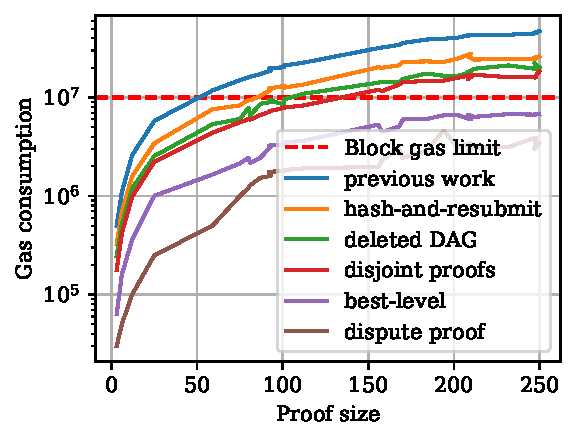
\includegraphics[width=1\columnwidth]{figures/dispute.pdf}
    \end{center}
    \caption{Caption}
    \label{fig:dispute}
\end{figure}

